\documentclass[11pt, twocolumn, a4paper]{article}

\usepackage{graphicx}
\usepackage{booktabs}
\usepackage{multirow}
\setlength{\oddsidemargin}{0.0 cm}
\setlength{\evensidemargin}{0.0 cm}
\setlength{\topmargin}{-1cm}
\setlength{\textheight}{24 cm}
\setlength{\textwidth}{16 cm}

\newcommand{\ttbarm}{\mathrm{t \overline{t} \; }}
\newcommand{\ttbar}{$\mathrm{t \overline{t} \; }$}
\newcommand{\ttbars}{${t \overline{t} \; }$}
\newcommand{\ttW}{{t \overline{t} W }}
\newcommand{\ttZ}{{t \overline{t} Z }}


\pagestyle{plain}

\setlength{\parindent}{0in}

\usepackage[
  locale=DE,
  separate-uncertainty=true,
  decimalsymbol=.,
  per-mode=symbol-or-fraction,
]{siunitx}
\DeclareSIUnit\permille{\text{\textperthousand}}
\usepackage{textcomp}
\usepackage{amsmath,amssymb}

\usepackage[verbose]{placeins}

\begin{document}
\thispagestyle{empty}

\author{Salvatore La Cagnina}

\title{Summary of `ATLAS Collaboration, {\it 'Measurement of the $t \overline{t} Z$ and $t \overline{t} W$ production cross sections in multilepton final states using $\SI{3.2}{fb^{-1}}$ of $pp$ collisions at $\sqrt{s} = \SI{13}{TeV}$ with the ATLAS detector'}}

\maketitle

In this paper a measurement of the $t \overline{t} Z$ and $t \overline{t} W$ production cross section is presented.
The sample contains $\SI{3.2}{fb^{-1}}$ of $pp$ collision data at $\sqrt{s} = \SI{13}{TeV}$.
The data is collected with the ATLAS detector at the LHC at CERN in the year 2015. 
In order to extract the cross sections, a maximum-likelihood fit is used at differently selected regions.\\
%
%
This measurement yields a test of the Standard Model (SM) due to new physics possibly changing the production of massive vector bosons together with \ttbars.
Furthermore, this measurement offers information about the neutral-current coupling of the top quark which can be compared to theoretical SM predictions.
This measurement has been previously studied for $7$ and $\SI{8}{TeV}$ \cite{paper_alt1,paper_alt2}, however, due to the increasing cross sections of processes this study is performed with higher center of mass energy.\\
%
%
For this measurement different decay channels are considered.
They can be separated in three different categories.
Those are same-sign muon (SS-$\mu$), trilepton and tetralepton.
The decay requirements for the channels and their correspondence to $\ttW$ and $\ttZ$ can be seen in Table \ref{tab:intro-channels}.
\begin{table}[htbp]
\centering
\caption{\label{tab:intro-channels} Decay modes with assignment to the $\ttW$ or $\ttZ$ process and analysis channel.\cite{paper}} 
\resizebox{0.5\textwidth}{!}{
\begin{tabular}{cccc}
\toprule
Process & \ttbar decay & Boson decay & Channel\\
\midrule
\multirow{2}{*}{$\ttW$} 
&  $(\mu^{\pm}\nu b) (q\bar{q} b) $ & $\mu^{\pm}\nu$ & SS dimuon\\
& $ (\ell^{\pm}\nu b) (\ell^{\mp}\nu b)$ & $\ell^{\pm}\nu$ & Trilepton\\
\midrule
\multirow{2}{*}{$\ttZ$} 
& $(\ell^{\pm}\nu b) (q\bar{q} b)$ & $ \ell^{+}\ell^{-}$ & Trilepton\\
& $(\ell^{\pm}\nu b) (\ell^{\mp} \nu b)$ & $ \ell^{+}\ell^{-}$ & Tetralepton\\
\bottomrule
\end{tabular}}
\end{table}
Each of the analysis channels is divided in multiple signal, control and validation regions.
For the cross sections the signal and control regions are fitted simultaneously.\\
%
%
The monte carlo samples are created using several generators with fixed top and Higgs masses to $m_t=\SI{172.5}{GeV}$ and $m_H=\SI{125}{GeV}.$
In order to correctly simulate the events the main backgrounds have to be implemented.
These are fake leptons, diboson events ($WZ,ZZ$) and other SM processes creating at least three prompt leptons like $Z$+jets or \ttbars + Higgs processes.\\
\FloatBarrier
%
Requiring leptons to be prompt and therefore being isolated reduces the amount of lepton background from hadron decays and misidentified leptons.
Other cuts and trigger requirement are also added in order to minimize the amount of background events.
For the different analysis channels and the different signal and control regions different cuts are applied.\\
The SS-$\mu$ channel has the highest sensitivity in comparison to other lepton channels due to the electron having a much higher charge misidentification.
The events are chosen by using cuts on the transverse momentum $p_T$, missing transverse momentum $E_T^{miss}$, the scalar sum of $p_T$ called $H_T$ and the number of $b$-tagged jets. 
The main background are fake leptons so the validation region is chosen to approve the background estimate which is extracted using the matrix method \cite{MM}.\\
%
In the trilepton channel four signal regions, one control region and two validation regions.
The signal regions are distinguished by their number of $b$-tagged and light jets, by the presence of a $Z$ candidate and the sign of two same flavor leptons.
This channel is sensitive to $\ttW$ and $\ttZ$ and its main background source is fake leptons but also other previously mentioned background.
The requirements of this channel which suppresses most other background are one pair of opposite signed same flavor leptons (OSSF) and the invariant mass of them being near the $Z$ mass.
This is valid for three of the four signal regions the last one having these requirements vetoed.
The validation regions are used to confirm the background hypothesis and the control region is used to constrain the $WZ$ background normalization for the fit.\\
%
The tetralepton channel is used for $\ttZ$ and requires two pairs of (OSSF) leptons.
Signal regions are chosen by the flavor of the pairs being identical or not and by the number of $b$-tagged jets leading to four different regions.
The main background is again cased by fake leptons and is suppressed by applying cuts on $p_T$, $H_T$ and the invariant mass of the opposite signed lepton pairs.
The control region is used to constrain the $ZZ$ background normalization for the fit analogously to the trilepton channel.\\
%
%
The main systematic uncertainties are caused by the reconstruction of the physics object and fake leptons (for $\ttW$), however, the main uncertainty for this measurement is the static uncertainties caused by the overall acceptance of the processes of $\SI{6}{\permille}$ and $\SI{2}{\permille}$ for $\ttZ$ and $\ttW$ respectively.\\
%
%
By simultaneously fitting the control and signal regions using a binned maximum-likelihood fit with systematic uncertainties as nuisance parameters, the cross sections can be extracted.
They are measured to be 
${\sigma_{\ttZ}=\SI[parse-numbers=false]{0.92 \pm 0.29 (stat.) \pm 0.10 (syst.)}{pb}}$ and 
${\sigma_{\ttW}=\SI[parse-numbers=false]{1.50 \pm 0.72 (stat.) \pm 0.33 (syst.)}{pb}}$.
These are consistent with the SM predictions which are calculated in NLO perturbative QCD to be
${\sigma_{\ttZ}=\SI[parse-numbers=false]{0.84 \pm 0.09}{pb}}$ and
${\sigma_{\ttW}=\SI[parse-numbers=false]{0.60 \pm 0.08}{pb}}$.
This can also be seen in fig. \ref{fig:theo} since the SM prediction is contained in the $\SI{68}{\%}$ confidence level interval.
Relying on this measurement the significance over the background only hypothesis for $\ttW$ is only $\si{2.2}\sigma$ which is not high enough to approve the existence of the $\ttW$ process.
The main reason is the high statistical uncertainty, therefore, further analysis with more data have to follow.
\begin{figure}[h!]
	\centering
	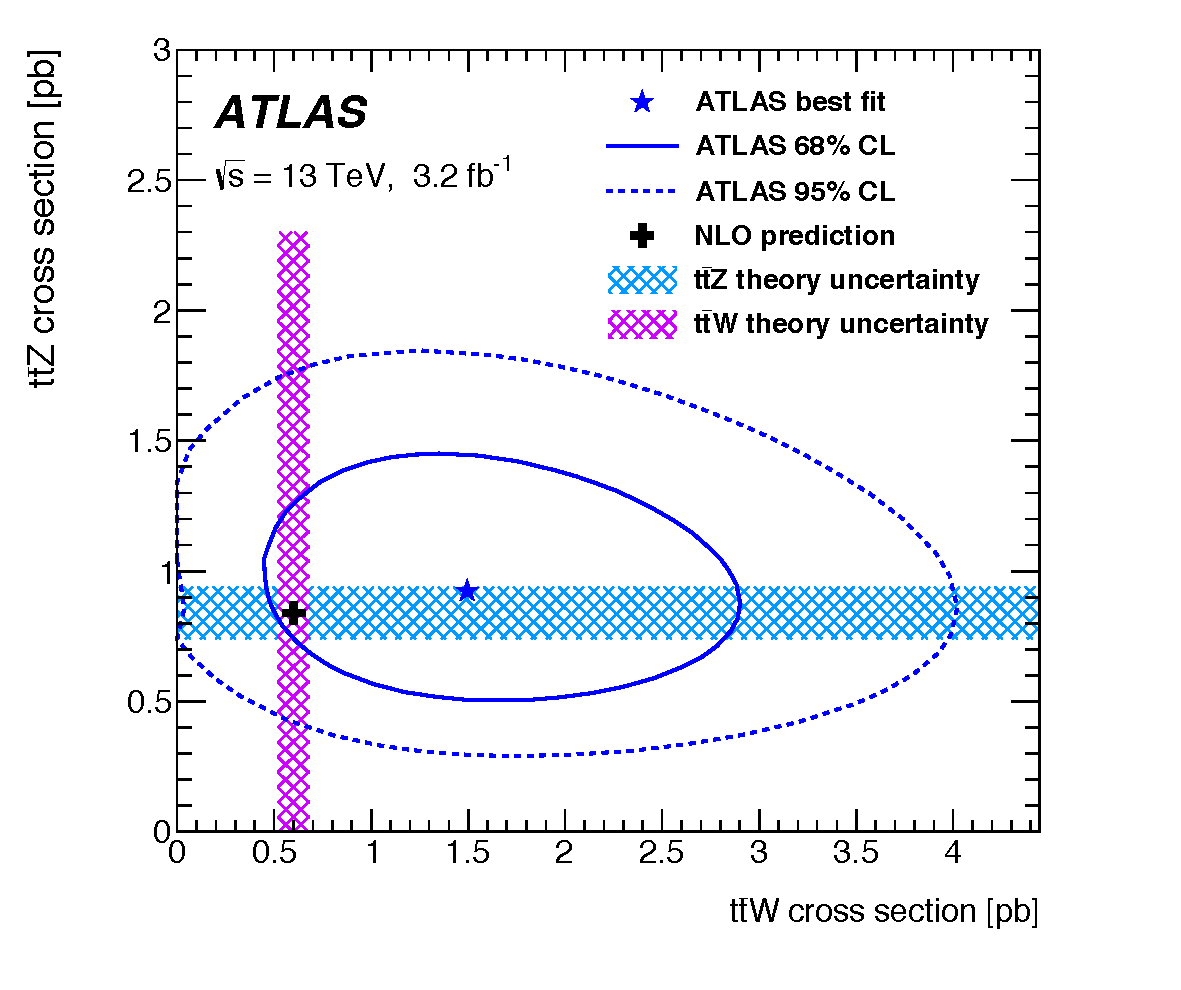
\includegraphics[width=0.5\textwidth]{paper/ttZ_vs_ttW_2Dfit.pdf}
	\caption{Resulting cross section for $\ttW$ and $\ttZ$ compared to the SM prediction. The $\SI{68}{\%}$ and $\SI{95}{\%}$ confidence level for the fit and the one sigma uncertainty for the theory is shown. \cite{paper}}
	\label{fig:theo}
\end{figure}

\begin{thebibliography}{99}
\bibitem{paper} ATLAS Collaboration,
Measurement of the $t \overline{t} Z$ and $t \overline{t} W$ production cross sections in multilepton final states using $\SI{3.2}{fb^{-1}}$ of $pp$ collisions at $\sqrt{s} = \SI{13}{TeV}$ with the ATLAS detector, Eur. Phys. J. C 77 (2017) 40.
\bibitem{paper_alt1} ATLAS Collaboration, 
Measurement of the $t \overline{t} W$ and $t \overline{t} Z$ production cross sections in $pp$ collisions at $\sqrt{s} = \SI{8}{TeV}$ with the ATLAS detector, JHEP 11 (2015) 172.
\bibitem{paper_alt2} CMS Collaboration, 
Observation of top quark pairs produced in association with a vector boson in $pp$ collisions at $\sqrt{s} = \SI{8}{TeV}$, JHEP 01 (2016) 096.
\bibitem{MM} ATLAS Collaboration, 
Measurement of the top quark-pair production cross section with ATLAS in $pp$ collisions at $\sqrt{s} = \SI{7}{TeV}$,
Eur. Phys. J. C 71 (2011) 1577.
\end{thebibliography}



\end{document}


%\begin{figure}[ht!]
%  \begin{center}
%    \includegraphics[width=0.5\textwidth]{plot.pdf}
%    \caption{A figure caption~\cite{brandt}.}
%    \label{fig:fig1}
%  \end{center}
%\end{figure}
